%****************************************************************************
%*  Autor: Nicolas Peter Lane                                               *
%*  Data: 02/04/2015                                                        *
%*  Modelo de monografia para TCC - UDESC conforme as normas da ABNT2       *
%*  sugest�es/d�vidas: lambdox@gmail.com                                    *
%*  									    *
%*  Licen�a GPL:              						    *
%*  Permission to use, copy, modify, and distribute this protocol and its   *
%*  documentation for any purpose, without fee, and without written         *
%*  agreement is hereby granted, provided that the above copyright notice,  *
%*  and the author appear in all copies of this protocol.                   *
%*                                                                          *
%****************************************************************************/

\documentclass[a4paper, ruledheader]{abnt}

\usepackage[brazilian]{babel} % Permite utilizar configuracoes da linguagem portugesa do Brasil e Inglesa
\usepackage[latin1]{inputenc} % Permite especificar codificacao das entradas (caracteres acentuados - � - sem usar \'a)
\usepackage{udesc}
\usepackage{graphicx}
\usepackage{latexsym}
\usepackage{psfrag}
\usepackage{subfig}
\usepackage{float}
\usepackage{amsmath}  %Permite usar f�rmulas matem�ticas
\usepackage{ragged2e} %Permite usar formata��o justificada /justify
\usepackage[Conny]{fncychap} 
\ChTitleAsIs

\begin{document}


\instituicao{UNIVERSIDADE DO ESTADO DE SANTA CATARINA - UDESC}
\centro{CENTRO DE CI�NCIAS TECNOL\'OGICAS - CCT}
\departamento{DEPARTAMENTO DE CI\^ENCIA DA COMPUTA\c{C}\~AO}
\curso{Gradua��o em CI\^ENCIA DA COMPUTA\c{C}\~AO}
\autor{DIGITE SEU NOME}
\titulo{DIGITE O T�TULO}
\orientador{Dr. Nome do Orientador}
\coorientador{Dr. Nome do Orientador} %comentar sen�o tiver co-orientador

\comentario{Trabalho de conclus�o de curso apresentado no curso de Ci\^encia da Computa\c{c}\~ao da Universidade Estadual 
de Santa Catarina, como requisito parcial para obten��o do grau de Ci\^encia da Computa��o.}

% Membros da comiss�o avaliadora
\bancaum{Prof. \ABNTorientadordata \\ \ABNTinstituicaodata \\ Orientador}
\bancadois{Prof. \ABNTcoorientadordata \\ Institui\c{c}\~ao\\ Co-orientador}%comentar sen�o tiver co-orientador                    
\bancatres{Prof. Dr. Nome do Convidado \\ Institui\c{c}\~ao}              
\bancaquatro{Prof. Dr. Nome do Convidado \\ Institui\c{c}\~ao}     

\local{Joinville-JLLE}
\data{m�s / ano}



\capa

\setcounter{page}{1} % inicia a contagem do numero das paginas
\pagenumbering{roman} % define tipo de numeracao romana minuscula
\folhaderosto


\termodeaprovacao
\vfill
\begin{flushright}
\hfill \textit{dedicatoria\\}
\end{flushright}

\vspace*{1cm}

\clearpage

\chapter*{Agradecimentos}
Dedico meus sincero agradecimentos para:

-- o professor Doutor..., pela orienta��o e incentivo

-- a equipe do laborat�rio ..., em especial pelos colegas ..., pela ajuda em diversos momentos.

\begin{resumo}

\begin{center}
 Resumo do Trabalho de Conclus�o de Curso apresentado � UDESC como parte dos requisitos necess�rios para obten��o do grau de Cientista da Computa��o.


{% Norma - fonte negrito, corpo 16
\bfseries
\LARGE

\ABNTtitulodata

}

\end{center}


\begin{singlespace}
	\noindent Orientador: \ABNTorientadordata\ \\
	\noindent Co-orientador: \ABNTcoorientadordata\ \\ %comentar sen�o tiver co-orientador
  \noindent Palavras-chave: Escreva; Aqui; Suas; Palavras-chave\\
\end{singlespace}


Escreva aqui o texto de seu resumo...




\end{resumo}



\begin{abstract}

\begin{center}

Abstract of bachelor monograph presented to UDESC as a partial fulfillment of the requirements for the degree of Computer Engineering.

{% Norma - fonte negrito, corpo 16
\bfseries
\LARGE

Title

}

\end{center}

\begin{singlespace}
  \noindent Advisor: \ABNTorientadordata \\
  \noindent Co-advisor: \ABNTcoorientadordata\\ %comentar sen�o tiver co-orientador
  \noindent Key words: Write; Here; Your; Key-words.\\
\end{singlespace}


Write here the English version of your `Resumo'...

\end{abstract}

% ====================================================================
% Contents
% ====================================================================
\tableofcontents

\listadesiglas

\listadesimbolos

% ====================================================================
% Contents
% ====================================================================
\listoffigures

% ====================================================================
% Contents
% ====================================================================
\listoftables


\setcounter{page}{0} % Reinicia a contagem do numero das paginas
\pagenumbering{arabic} % Numeracao dos capitulos arabica


% ************* TEXTO *************
% A parte textual deve conter:
% 1 - Introdu��o
% 2 - Revis�o de Literatura
% 3 - Material e M�todos
% 4 - An�lise dos Resultados
% 5 - Discuss�o
% 6 - Conclus�o
\chapter{Introdu��o}
\label{cap:introducao1}


A acessibilidade � a possibilidade de qualquer pessoa, independentemente de suas capacidades f�sico-motoras e perceptivas, culturais e sociais, usufruir os benef�cios de uma vida. Al�m disso, a acessibilidade tem como objetivo possibilitar o acesso de pessoas com defici�ncia permanente ou tempor�ria (e.g., f�sicas, auditivas, etc.) na sociedade afim de que todas possam participar ativamente.

Para que o objetivo da acessibilidade seja cumprido, � necess�rio o estudo e cria��o de alternativas, para que estas pessoas possam contornar ou compensar algum tipo de defici�ncia que as impe�a a sua inser��o. Essa demanda motivou o surgimento da \acf{TA}, uma parte da tecnologia que deve ser entendida como um aux�lio que promove a amplia��o de uma habilidade funcional deficit�ria ou possibilitar a realiza��o da fun��o desejada e que se encontra impedida. Contudo, ainda s�o encontradas muitas dificuldades, principalmente pelo tema ser consideravelmente novo, a quantidade de trabalhos cient�ficos relacionado ao tema ainda � pouco expressivo.

Nas diferentes classifica��es da \ac{TA}, existe a \acf{CAA} que pode ser definida como uma alternativa a comunica��o escrita e oral. A \ac{CAA} inicialmente era composta apenas de sistemas sem tecnologia, como libras, cart�es e livros. Por�m, com o avan�o da tecnologia nas �ltimas d�cadas, sistemas anal�gicos e sistemas com recursos computacionais foram aumentando o escopo e as alternativas de \ac{CAA}.

Com uma quantidade expressiva de pessoas com algum tipo de paralisia no Brasil e no mundo, meios alternativos de inclus�o s�o necess�rios, principalmente meios alternativos dispon�veis a popula��o com baixa renda. Um dos objetivos espec�ficos do trabalho � analisar e diferenciar solu��es de \ac{CAA} que possibilitam a estimula��o cognitiva de pessoas com \acf{PC} em especial as pessoas que possuem habilidades locomotoras limitadas em conjunto com dificuldades na fala. Ap�s esta an�lise, verificar se � necess�ria a implementa��o de uma solu��o alternativa a essas pessoas. Contudo, esta s� pode ser atingida atrav�s de estudos sobre \ac{PC} e os requisitos que estas solu��es demandam. O principal objetivo do trabalho resume-se em implementar um software para computador alternativo de \ac{CAA} de licen�a GPL, para que pessoas com \ac{PC} possam ter seus c�rebros estimulados cognitivamente. 

A organiza��o deste trabalho est� dividida em quatro cap�tulos, ``Conceitos B�sicos'', ''Defini��o do Problema'', ``Proposta'' e ``Considera��es''. No primeiro cap�tulo s�o apresentados a quantidade de pessoas com defici�ncia no Brasil e no mundo, defini��es e legisla��o sobre \ac{TA} e \ac{TA} dentro da inform�tica, tamb�m � abordado as pessoas que possuem \ac{PC} e seus diferentes casos. Al�m disso, tamb�m estuda-se as principais iniciativas de \ac{TA} pelo mundo e seus termos e classifica��es. Ao final do cap�tulo � apresentado as defini��es de \ac{CAA} os seus recursos e estrat�gias e quais os termos e classifica��o que ser�o utilizados no trabalho.

No segundo cap�tulo, � definido o problema e os usu�rios finais da solu��o. O trabalho nesta parte levanta problemas com a prancha de comunica��o, que � a solu��o atual dos terapeutas, e ap�s isso identifica os requisitos necess�rios para o desenvolvimento da solu��o atrav�s de entrevista com uma psic�loga especialista em reabilita��o de pessoas com \ac{PC}. Ao final s�o identificados trabalhos correlatos e apresentado uma compara��o com base nos requisitos levantados.

No terceiro cap�tulo, � elaborado uma especifica��o da proposta, determinando os m�todos que ser�o utilizados para cumprir os requisitos levantados. Atrav�s de diagramas das tarefas, diagramas de classe e de estados da solu��o o trabalho indica quais ser�o as intera��es do usu�rio com a solu��o. S�o mencionados tamb�m os limitadores e e plano de teste que tem como objetivo fazer com que a solu��o evolua no decorrer do trabalho. 

\chapter{Conceitos}
\label{cap:introducao}
\acresetall
Ao longo da hist�ria em rela��o �s pessoas com defici�ncia, � poss�vel encontrar uma variedade de termos que foram se modificando ao longo dos anos: ``Inv�lidos'', ``incapacitados'', ``defeituosos'', ``excepcionais'' s�o alguns exemplos de termos atribu�dos �s pessoas com defici�ncia em diferentes �pocas. Os termos s�o considerados corretos em fun��o de valores e conceitos vigentes em cada sociedade e em cada �poca, portanto, os termos supracitados foram aceitos, usados e, em dados momentos da hist�ria, substitu�dos. No estudo da evolu��o do conceito da defici�ncia encontra-se que, em 1980, a Organiza��o Mundial de Sa�de prop�s a utiliza��o da CIDID - Classifica��o das Defici�ncias, Incapacidades e Desvantagens\cite{cidid} ({\it Handicaps})\footnote{Termo em ingl�s traduzido como defici�ncia} com intuito de organizar uma linguagem universal a respeito das defici�ncias. A implementa��o de uma nova terminologia, ``pessoas deficientes'', passou a atribuir o valor de pessoa a aqueles que at� ent�o eram desconsiderados como tais pela sociedade. Ressalta-se que a revis�o dessas nominatas teve a preocupa��o de centrar-se na pessoa e n�o na defici�ncia \cite{fiquene,chagas}.

Segundo a \citeonline{onu}, existem no mundo 1 bilh�o de pessoas que possuem algum tipo de defici�ncia. Segundo o Censo de 2010 \cite{censo} a ocorr�ncia de pessoas com defici�ncia na popula��o brasileira � de 23,9\% da popula��o. A tabela \ref{tabela_pop} apresenta a distribui��o dos tipos de defici�ncia no Brasil.


\begin{table}[bth!]
\centering
\scriptsize
\caption{Distribui��o dos tipos de defici�ncia no Brasil.}\vspace{.2cm}

	
    \begin{tabular}{ | l | l |}
		
    \hline
    Condi��o & Por��o da Popula��o\\ \hline \hline
    Defici�ncia Visual & 18,6\%\\ \hline
		Defici�ncia Motora & 7\%\\ \hline
		Defici�ncia Auditiva & 5,1\%\\ \hline
		Defici�ncia Mental ou Intelectual & 1,4\%\\ \hline
		
    \end{tabular}
    \label{tabela_pop}
		\vspace{0.1cm}\\Fonte: o pr�prio autor com base no Censo de 2010\cite{censo}.

\end{table}



A tabela \ref{tabela_pop} mostra que na popula��o brasileira, 18,6\% da popula��o possuem defici�ncia visual sendo a defici�ncia mais recorrente entre os brasileiros. A defici�ncia motora, a segunda com maior recorr�ncia, � apresentada em 7\% da popula��o, seguida da defici�ncia auditiva com 5,1\%, e das pessoas com defici�ncia mental que apresentam 1,4\%. Na tabela \ref{tabela_pop} a soma das porcentagens n�o � igual a 23,9\% pois algumas pessoas possuem mais de uma defici�ncia citada. Outro fator importante � que 65\% das pessoas que possuem algum tipo de defici�ncia recebem menos de dois sal�rios m�nimos no Brasil\cite{censo}, sendo que 10\% dessas pessoas tem renda de menos da metade de um sal�rio m�nimo. 

As pessoas que possuem algum tipo de defici�ncia sofrem dificuldades ao acesso das necessidades b�sicas conquistadas pelo ser humano, segundo o Programa de A��o Mundial para Pessoas Deficientes da ONU\cite[p.~11]{onu},

\begin{quotation}''[...] a experi�ncia tem demonstrado que, em grande medida, � o meio que determina o efeito de uma
incapacidade sobre a vida cotidiana da pessoa. A pessoa v�-se relegada � invalidez quando
lhe s�o negadas as oportunidades de que disp�e, em geral, a comunidade, e que s�o
necess�rias aos aspectos fundamentais da vida, inclusive a vida familiar, a educa��o, o
trabalho, a habita��o, a seguran�a econ�mica e pessoal, a participa��o em grupos sociais e
pol�ticos, as atividades religiosas, os relacionamentos afetivos e sexuais, o acesso �s
instala��es p�blicas, a liberdade de movimenta��o e o estilo geral da vida di�ria [...]''.
\end{quotation} 

Neste trabalho � dada �nfase a pessoas com defici�ncia motoras, mais especificamente as pessoas que possuem \ac{PC}.  A Encefalopatia Cr�nica da Inf�ncia (E.C.I.), tamb�m conhecida como \ac{PC}, � uma doen�a cr�nica de car�ter n�o evolutivo, que em 90\% das vezes possuem defici�ncia f�sica. O curso natural das les�es � de longa dura��o, necessitando a crian�a de tratamento prolongado. Tem efeitos n�o apenas sobre o crescimento e o desenvolvimento f�sico, mas tamb�m sobre a destreza, a personalidade, a capacidade cognitiva, as atitudes pessoais e sociais do paciente, as emo��es e as intera��es da fam�lia\cite{leite,sa}. Como a \ac{PC} possui diferentes tipos de manifesta��es e graus da doen�a, para maior compreendimento das necessidades de pessoas com \ac{PC}, � necess�rio conhecer os diferentes quadros cl�nicos da doen�a. 


\section{Quadro Cl�nico: \acf{PC}}

Existem v�rios quadros cl�nicos de pessoas, que possuem \ac{PC}, e podem ser beneficiadas por algum recurso que facilite a sua comunica��o com outras pessoas. Neste sentido alguns quadros se encaixam melhor ou pior a determinadas facilidades de comunica��o. As poss�veis causas da \ac{PC} (e.g., causas pr�-natais, perinatais e p�s-natais) n�o ser�o tratadas, pois n�o pertencem ao escopo deste trabalho.
Na observa��o cl�nica da \ac{PC}, deve-se levar em considera��o a extens�o do dist�rbio motor, sua intensidade e, principalmente, a caracteriza��o semiol�gica\footnote{Caracteriza��o semiol�gica, refere-se a caracteriza��o dos sinais e sintomas da doen�a.} desse dist�rbio\cite{leite}. Assim, a paralisia cerebral apresenta v�rias formas cl�nicas que s�o apresentadas na tabela \ref{tabela}.

\begin{table}[bth!]
\centering
\scriptsize
\caption{Tabela com os diferentes casos de \ac{PC}.}\vspace{.2cm}

	
    \begin{tabular}{ | l |  p{7cm} | p{5cm} |}
		
    \hline
    Quadro & Descri��o das Limita��es  & Aplic�vel recurso de comunica��o\\ \hline \hline
    Hemiplegia &   Sinais de libera��o tais como espasticidade , hiper reflexia e sinal de Babinski & Aplic�vel em alguns graus \\ \hline
    Hemiplegia bilateral & Tetra ou quadriplagia, dependendo do grau defici�ncia mental e epilepsia & Aplic�vel a pacientes com menor grau de les�o \\ \hline
    Diplegia & Com\-pro\-me\-ti\-men\-to dos membros inferiores, co\-mu\-men\-te evidenciando uma acentuada hipertonia dos adutores & Aplic�vel em alguns graus \\
    \hline
		Discinesia & Movimentos involunt�rios, ondulantes e repetidos com grande amplitude de movimento e incoordena��o motora &  Aplic�vel em alguns graus \\
    \hline
		Ataxia &  Perda de coordena��o dos movimentos musculares volunt�rios & Aplic�vel em alguns graus \\
    \hline
		Formas mistas & Combina��o dos quadros anteriores & Casos avaliados individualmente \\
    \hline
		
    \end{tabular}
    \label{tabela}
		Fonte: o pr�prio autor com base \citeonline{leite}.

\end{table}


A Tabela {\ref{tabela}} apresenta os diferentes quadros de \ac{PC}. Atrav�s dela pode-se perceber que independente do quadro, o grau da les�o de cada paciente com \ac{PC} tem que ser avaliado individualmente, para que se identifique quais s�o as necessidades de acessibilidade de cada um deles.  Para maiores informa��es sobre cada quadro cl�nico, ver Ap�ndice {\ref{apendice1}.



%No Brasil existem diversos movimentos sociais, dos mais variados �mbitos,voltados a ajudar as pessoas com defici�ncias. Tratando-se das pessoas com \ac{PC} os movimentos sociais tamb�m s�o decisivos. No entanto, os recursos normas e leis de acessibilidade ainda que claros, s�o parcialmente esquecidos pela sociedade e pela falta de investimento e pesquisa na �rea.As dificuldades encontradas s�o grandes, pois s�o poucas as literaturas especializadas e faltam equipamentos acess�veis a esse grupo da popula��o.

\section{Acessibilidade}

A acessibilidade � a possibilidade de qualquer pessoa, independentemente de suas capacidades f�sico-motoras e perceptivas, culturais e sociais, usufruir os benef�cios de uma vida em sociedade. � a possibilidade de participar de todas as atividades, at� as que incluem o uso de produtos, servi�os e informa��o, com o m�nimo de restri��es poss�vel \apud{nicholl,nbr}{unirio}.

As discuss�es sobre acessibilidade v�m crescendo no Brasil e no mundo \cite{donatangelo}.
O termo acessibilidade � muito amplo e, de certa forma, complexo de ser definido,
pois n�o pode ser entendido apenas como a facilidade de se ter acesso. Contudo, pode-se
caracterizar, de um modo geral, acessibilidade como sendo um processo din�mico que visa �
elimina��o de barreiras para que se tenha acesso.

A acessibilidade tamb�m � conhecida por ser a possibilidade e condi��o de alcance para a utiliza��o, com autonomia, simplicidade, efici�ncia e seguran�a, dos espa�os, mobili�rios, das edifica��es, dos equipamentos urbanos, dos transportes, dos sistemas e meios
de comunica��o e da inform�tica, por qualquer pessoa, sejam elas crian�as, adultos, idosos, contendo, ou n�o, necessidades especiais devido alguma defici�ncia ou mobilidade reduzida \apud{torres}{donatangelo}. No Brasil h� legisla��o que trata de quest�es de acessibilidade aos portadores de necessidades especiais. A legisla��o mais relevante no contexto deste trabalho s�o:
\begin{itemize}
\item Portaria n� 1.679, de dezembro de 1999, disp�e sobre requisitos de acessibilidade de 
pessoas portadoras de defici�ncias, para instruir os processos de autoriza��o e de 
reconhecimento de cursos, e de credenciamento de institui��es. 
 \cite{mec};
\item Lei n� 10.098, de dezembro de 2000, que, entre outras coisas, estabelece
normas gerais e crit�rios b�sicos para que seja promovida a acessibilidade
para pessoas com defici�ncia \cite{brasil}; e
\item Decreto n� 3.294, de dezembro de 1999, que instituiu o programa
Sociedade da Informa��o, na qual um dos objetivos � a universaliza��o do
acesso � Internet \cite{brasil1}.
\end{itemize}


Com a legisla��o presente, principalmente pelo decreto n� 3.294 a Acessibilidade ultrapassa as barreiras do espa�o f�sico e chega ao espa�o digital. No espa�o digital s�o encontradas muitas dificuldades, entre elas podem ser citadas a falta de
recursos tecnol�gicos, a falta de acesso aos recursos existentes e a falta de preocupa��o em
disponibilizar a informa��o de forma clara\apud{torres1}{donatangelo}. A utiliza��o de dispositivos eletr�nicos (e.g., computadores, {\it tablets} e { \it smart\-pho\-nes}) e o acesso � Internet permitem aos cidad�os acessarem um conjunto consider�vel de fontes de informa��o, estabelecerem contatos e trocarem
informa��es, exercerem uma atividade social e encontrarem formas alternativas de lazer e de
divertimento \apud{abra}{donatangelo}. Para que ocorra o mesmo com pessoas portadoras de algum tipo de defici�ncia, a acessibilidade na inform�tica � necess�ria.



\subsection{Acessibilidade na Inform�tica}

Para que a acessibilidade na inform�tica ocorra, � necess�rio levar em considera��o a redund�ncia, a simplicidade e a facilidade para compreens�o da informa��o\cite{torres}. A web desempenha um papel fundamental no avan�o que a Internet representa no cotidiano das pessoas com defici�ncia, facilitando a vida deles; ela permite que eles criem novas formas de relacionamento, encontrem oportunidades de trabalho e formas alternativas de divers�o \cite{torres}.

Atualmente a maioria dos web sites t�m barreiras de acessibilidade que dificultam ou mesmo tornam imposs�vel para estas pessoas acessarem sites. Contudo, se os web sites e softwares forem projetados levando em considera��o a acessibilidade, estas pessoas poder�o usar os sites efetivamente\cite{wc}.

Em maio de 1999 os membros do \ac{W3C} elaboraram o ``Estatuto de Recomenda��o do \ac{W3C}'' (WCAG 1.0), esse documento constitui a primeira vers�o das Diretrizes para a Acessibilidade ao Conte�do da web. Al�m disso, no Brasil o governo disponibiliza em seu site oficial o \ac{eMAG} \cite{emag} que consiste em um conjunto de recomenda��es a ser considerado para que o processo de acessibilidade dos sites e portais do governo brasileiro seja conduzido de forma padronizada e de f�cil implementa��o. O \ac{eMAG} � coerente com as necessidades brasileiras e em conformidade com os padr�es internacionais. Foi formulado para orientar profissionais que tenham contato com publica��o de informa��es ou servi�os na Internet a desenvolver, alterar e ou adequar p�ginas, web sites e portais, tornando-os acess�veis ao maior n�mero de pessoas poss�vel. 

Apesar de importante, a acessibilidade digital e na web n�o � t�o simples \cite{harrison}. Por exemplo, pessoas com defici�ncia possuem limita��es sensoriais e motoras que devem ser compensadas de alguma forma, a fim de viabilizar o acesso dessas pessoas aos recursos computacionais e, para isso, as organiza��es necessitam adaptar seu hardware e seus sistemas, a fim de fazer com que um computador possa ser usado por pessoas com defici�ncia \cite{harrison}. 

A acessibilidade digital, faz com que pessoas, que possuem algum tipo de defici�ncia, tenham acesso ao conte�do disponibilizado na web. Por�m, ainda existem barreiras em web sites, softwares, e algumas defici�ncias fazem com que as pessoas tenham limita��es sensoriais e/ou motoras. Sendo assim, � necess�rio um meio de compensar estas dificuldades para garantir o acesso a essas informa��es.


\section{Tecnologia Assistiva}
\label{Tecnologia Assistiva}

O termo {\it Assistive Technology}, traduzido no Brasil como \ac{TA} ou tamb�m conhecido como Ajudas T�cnicas, foi adotado no Brasil ap�s ser criado em 1988, como importante elemento jur�dico dentro da legisla��o norte-americana conhecida como {\it Public Law 100-407} e foi renovado em 1998 com o {\it Assistive Technology Act} de 1998. Comp�e, com outras leis, o \ac{ADA}, que regula os direitos dos cidad�os com defici�ncia nos Estado Unidos da Am�rica, al�m de regulamentar o uso de verbas para incentivos e projetos de aux�lio a pessoas com defici�ncias \cite{romeu,lima}.

A \ac{TA} deve ser entendida como um aux�lio que promove a amplia��o de uma habilidade funcional deficit�ria ou possibilitar a realiza��o da fun��o desejada e que se encontra impedida por circunst�ncia de defici�ncia, limita��es ou pelo envelhecimento. A \ac{TA} est� inserida como uma diretriz da tecnologia, possibilitando que pessoas com defici�ncia possam interagir com  a sociedade n�o apenas se comunicando, mas participando ativamente do meio em que vivem \cite{radabaugh,bersch}. Para que esses objetivos sejam alcan�ados o servi�o de Tecnologia Assistiva necessita contemplar\cite{bersch}:
\begin{itemize}
\item A avalia��o do caso cl�nico de cada paciente;
\item A sele��o do recurso mais apropriado a cada caso;
\item O ensino do usu�rio sobre a utiliza��o de seu recurso;
\item O acompanhamento durante a implementa��o da TA no contexto de vida real; e
\item As reavalia��es e ajustes no processo. 
\end{itemize}

Como existem v�rios recursos de \ac{TA} no mercado, � atribui��o do prestador de servi�o de \ac{TA} conhecer e orientar o usu�rio quanto aos recursos gratuitos e oferecidos pelo governo, e recursos particulares, os oferecidos por empresas que atuam no desenvolvimento de recursos de \ac{TA}. A equipe de profissionais envolvidos na coordena��o do servi�o de TA pode variar, dependendo da caracter�stica deste servi�o, da modalidade de TA que se � proposto a orientar e colocar em pr�tica, e tamb�m do local o qual o paciente est� inserido\cite{bersch}:

\begin{itemize} 
\item Sala de recursos multifuncionais dentro de uma escola;
\item Centro de reabilita��o;
\item Universidade com servi�o especializado e pesquisa na �rea da comunica��o alternativa;
\item Servi�o de arquitetura especializado em acessibilidade ambiental;
\item Centro formador de para-atletas; e
\item Um servi�o de reabilita��o profissional. 
\end{itemize}

A \ac{TA} engloba as �reas de \ac{CAA}, mobilidade alternativa, adapta��es ao acesso ao computador,  equipamentos de aux�lio a vis�o e au\-di\-��o, a\-da\-pta\-��es de jogos e brincadeiras, adapta��es da postura sentada, pr�teses e a integra��o dessa tecnologia nos diferentes ambientes (e.g., casa, escola e trabalho)\apud{gill}{pelosi1}. O Brasil utiliza as diretrizes da \ac{ADA} como base para a classifica��o de \ac{TA}, e utiliza tamb�m a classifica��o da norma ISO 9999:2011(Anexo~\ref{iso9999}), por�m o \ac{CAT} concluiu que n�o existe uma �nica forma de classificar Tecnologia Assistiva. As v�rias classifica��es existentes s�o aplicadas de acordo com os objetivos de cataloga��o de recursos, ensino, trocas de informa��o, organiza��o de servi�os de aconselhamento e concess�o \cite{corde}. O importante � ter claro o conceito de \ac{TA} supracitada e os objetivos para os quais as classifica��es foram criadas. Existem diferentes tipos de equipamentos para aux�lio de pessoas com defici�ncia separados em algumas categorias pelas diretrizes da \ac{ADA} \cite{pelosi1}:

\label{classificacao}

\vspace{.5cm}

\begin{enumerate}
\item{Aux�lio para o dia a dia (e.g., comer, cozinhar e tomar banho). A figura \ref{fig:talher} � um exemplo de dois talheres para pessoas com defici�ncia.
\vspace{.5cm}

\begin{figure}[bth!]
  \begin{center}
    \caption{Exemplo de talher assistivo}\vspace{.2cm}
			
      \centering
      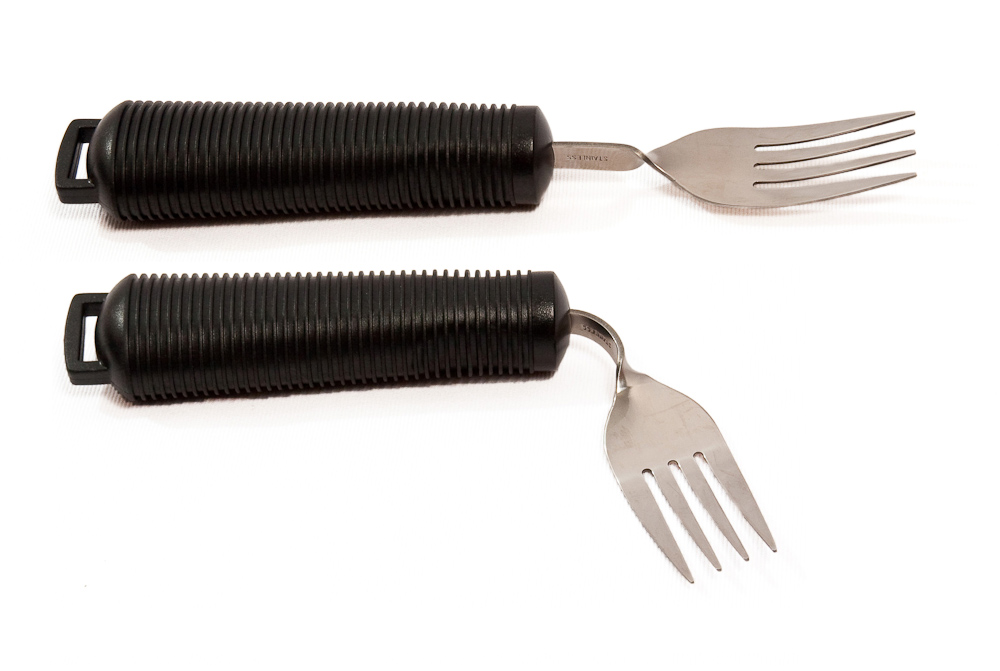
\includegraphics[width=5cm]{../figuras/talher.jpg}\\
			Fonte:\cite{vivere}
    
    \label{fig:talher}
  \end{center}
\end{figure}

A Figura \ref{fig:talher} mostra dois talheres que possuem cabos maiores para facilitar o manuseio, e um deles � ``dobrado'' para facilitar o posicionamento dos mesmos. Pacientes com quadros apresentados de Hemiplegia, Diplegia e algumas formas mistas podem se beneficiar com este tipo de talher.

}
\item{\acf{CAA}. Recursos eletr�nicos ou n�o para pessoas sem fala ou com limita��es dela (e.g., pranchas de comunica��o, vocalizadores, e softwares). A Figura \ref{fig:prancha} � um exemplo de prancha de comunica��o.

\begin{figure}[bth!]
  \begin{center}
    \caption{Exemplo de prancha de comunica��o}\vspace{.2cm}
			
      \centering
      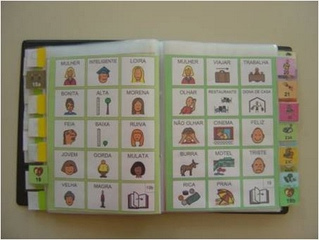
\includegraphics[width=5cm]{../figuras/prancha.jpg}\\
			Fonte:\cite{assistiva}
    
    \label{fig:prancha}
  \end{center}
\end{figure}

As pranchas de comunica��o exemplificadas na Figura \ref{fig:prancha} s�o meios de comunica��o para as pessoas com fala comprometida, isso pode ocorrer em todos os casos cl�nicos da \ac{PC}.

}
\item{Acessibilidade ao computador (e.g., teclados modificados, leitor de tela e ampliador de tela). A Figura \ref{fig:teclado} � um exemplo de teclado em modificado.
\vspace{-.5cm}
\begin{figure}[bth!]
  \begin{center}
    \caption{Exemplo de teclado em braile }\vspace{.2cm}
			
      \centering
      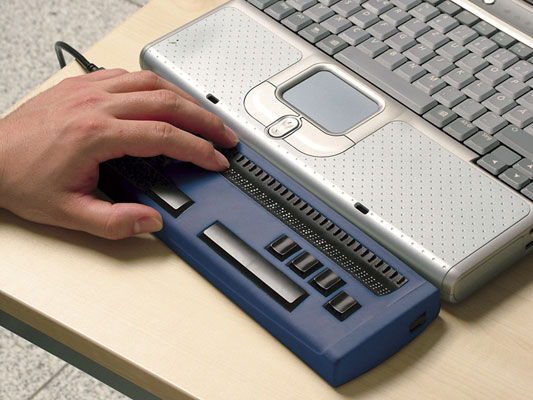
\includegraphics[width=4cm]{../figuras/teclado.jpg}\\
			Fonte:\cite{teclado}
    
    \label{fig:teclado}
  \end{center}
\end{figure}

A Figura \ref{fig:teclado} mostra que nos teclados modificados, a impress�o do que referencia cada tecla � na verdade um s�mbolo usado no alfabeto braile.

}
\item{Sistemas de controle de ambientes, que permitem que pessoas com dificuldades motoras controlem equipamentos a dist�ncia. A Figura \ref{fig:controle} � um exemplo de controle remoto para cegos.
\vspace{-.5cm}

\begin{figure}[bth!]
  \begin{center}
    \caption{Exemplo de controle assistivo}\vspace{.2cm}
			
      \centering
      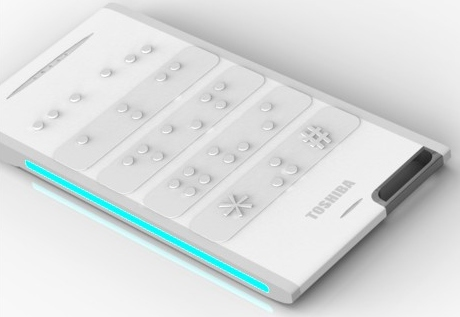
\includegraphics[width=4cm]{../figuras/controle.jpg}\\
			Fonte:\cite{controle}
    
    \label{fig:controle}
  \end{center}
\end{figure}
}
\vspace{-.5cm}
A Figura \ref{fig:controle} � um controle remoto que ao inv�s de possuir teclas com desenhos das fun��es e n�meros, os bot�es s�o representados em braile, para que os cegos possam manipular objetos a dist�ncia.

\item{Projetos Arquitet�nicos (e.g., cal�adas com guia para cegos e rampas de acesso). A Figura \ref{fig:rampa} � um exemplo de ramapa de acesso.

\begin{figure}[bth!]
  \begin{center}
    \caption{Exemplo de rampa de acesso}\vspace{.2cm}
			
      \centering
      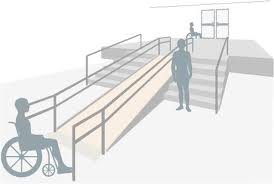
\includegraphics[width=4cm]{../figuras/rampa.jpg}\\
			Fonte:\cite{portal}
    
    \label{fig:rampa}
  \end{center}
\end{figure}

A Figura \ref{fig:rampa} representa uma rampa de acesso a cadeirantes, que torna poss�vel ao cadeirante o acesso a lugares mais elevados sem utilizar a ajuda de outras pessoas.

}
\item{�rteses e pr�teses, que permitem a troca ou ajuste de um membro. A Figura \ref{fig:protese} � um exemplo de pr�tese.
\vspace{-.5cm}
\begin{figure}[bth!]
  \begin{center}
    \caption{Exemplo de pr�tese}\vspace{.2cm}
			
      \centering
      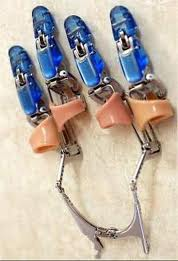
\includegraphics[width=3cm]{../figuras/protese.jpg}\\
			Fonte:\cite{protese}
    
    \label{fig:protese}
  \end{center}
\end{figure}
\vspace{-.5cm}
As pr�teses exemplificadas na Figura \ref{fig:protese}, ajudam as pessoas com membros danificados ou perdidos, a reabilita��o de movimentos.

}
\item{Equipamentos de aux�lio a postura (e.g., almofadas anat�micas e cintos). A Figura \ref{fig:cadeira} � um exemplo de cadeira de rodas com ajuste de postura.
\vspace{.5cm}
\begin{figure}[bth!]
  \begin{center}
    \caption{Exemplo de cadeira com regulagem de postura}\vspace{.2cm}
			
      \centering
      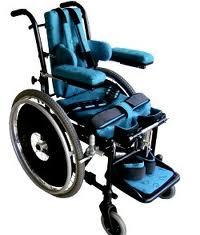
\includegraphics[width=4cm]{../figuras/cadeira.jpg}\\
			Fonte \cite{cadeira}
    
    \label{fig:cadeira}
  \end{center}
\end{figure}
}

Na Figura \ref{fig:cadeira} � poss�vel perceber o cinto na cadeira de rodas, que regulam a postura da pessoas do usu�rio.

\item{Equipamentos de mobilidade (e.g., cadeira de rodas motorizadas ou n�o e andadores). A Figura \ref{fig:cadeiramotorizada} representa um exemplo de cadeira de rodas motorizada.
\vspace{2cm}
\begin{figure}[bth!]
  \begin{center}
    \caption{Exemplo de cadeira de rodas motorizadas}
			
      \centering
      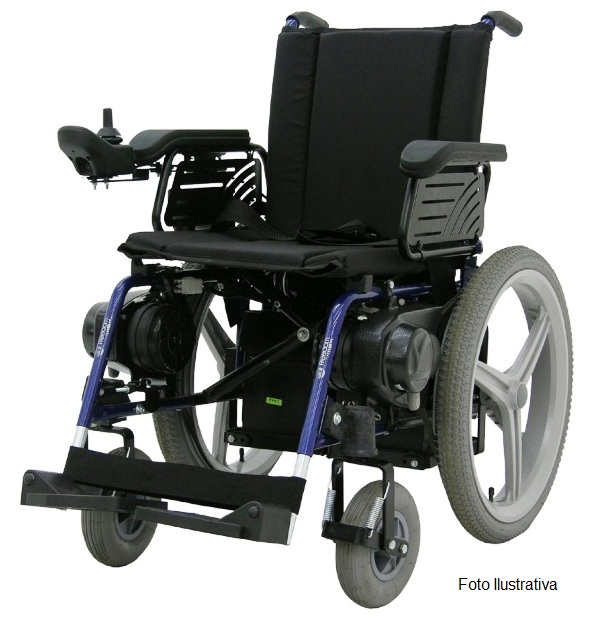
\includegraphics[width=3.5cm]{../figuras/cadeiramotorizada.jpg}\\
			Fonte: \cite{cinta}
    
    \label{fig:cadeiramotorizada}
  \end{center}
\end{figure}

Na Figura \ref{fig:cadeiramotorizada}, a cadeira possui um motor el�trico que faz com que a pessoa que a utiliza n�o necessite de grande esfor�o f�sico para moviment�-la.


}
\item{Aux�lio de surdos ou com audi��o parcial (e.g., aparelhos de surdez e telefones com teclado). A Figura \ref{fig:aparelhosurdez} � um exemplo de aparelho de surdez.
\vspace{-.5cm}
\begin{figure}[bth!]
  \begin{center}
    \caption{Exemplo de aparelho de surdez}
			
      \centering
      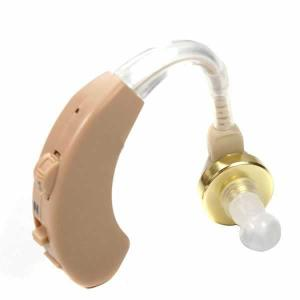
\includegraphics[width=3.5cm]{../figuras/aparelhosurdez.jpg}\\
			Fonte: \cite{surdez}
    
    \label{fig:aparelhosurdez}
  \end{center}
\end{figure}
}
\vspace{-.5cm}

Os aparelhos de surdez ilustrados pela Figura \ref{fig:aparelhosurdez} possibilitam que o �udio seja amplificado para que pessoas com defici�ncia auditiva parcial, possam escutar normalmente.

\item{Adapta��es a ve�culos. A Figura \ref{fig:carro} � um exemplo de carro adaptado a pessoas com defici�ncias f�sicas.
\begin{figure}[bth!]
  \begin{center}
    \caption{Exemplo de carro adaptado}\vspace{.2cm}
			
      \centering
      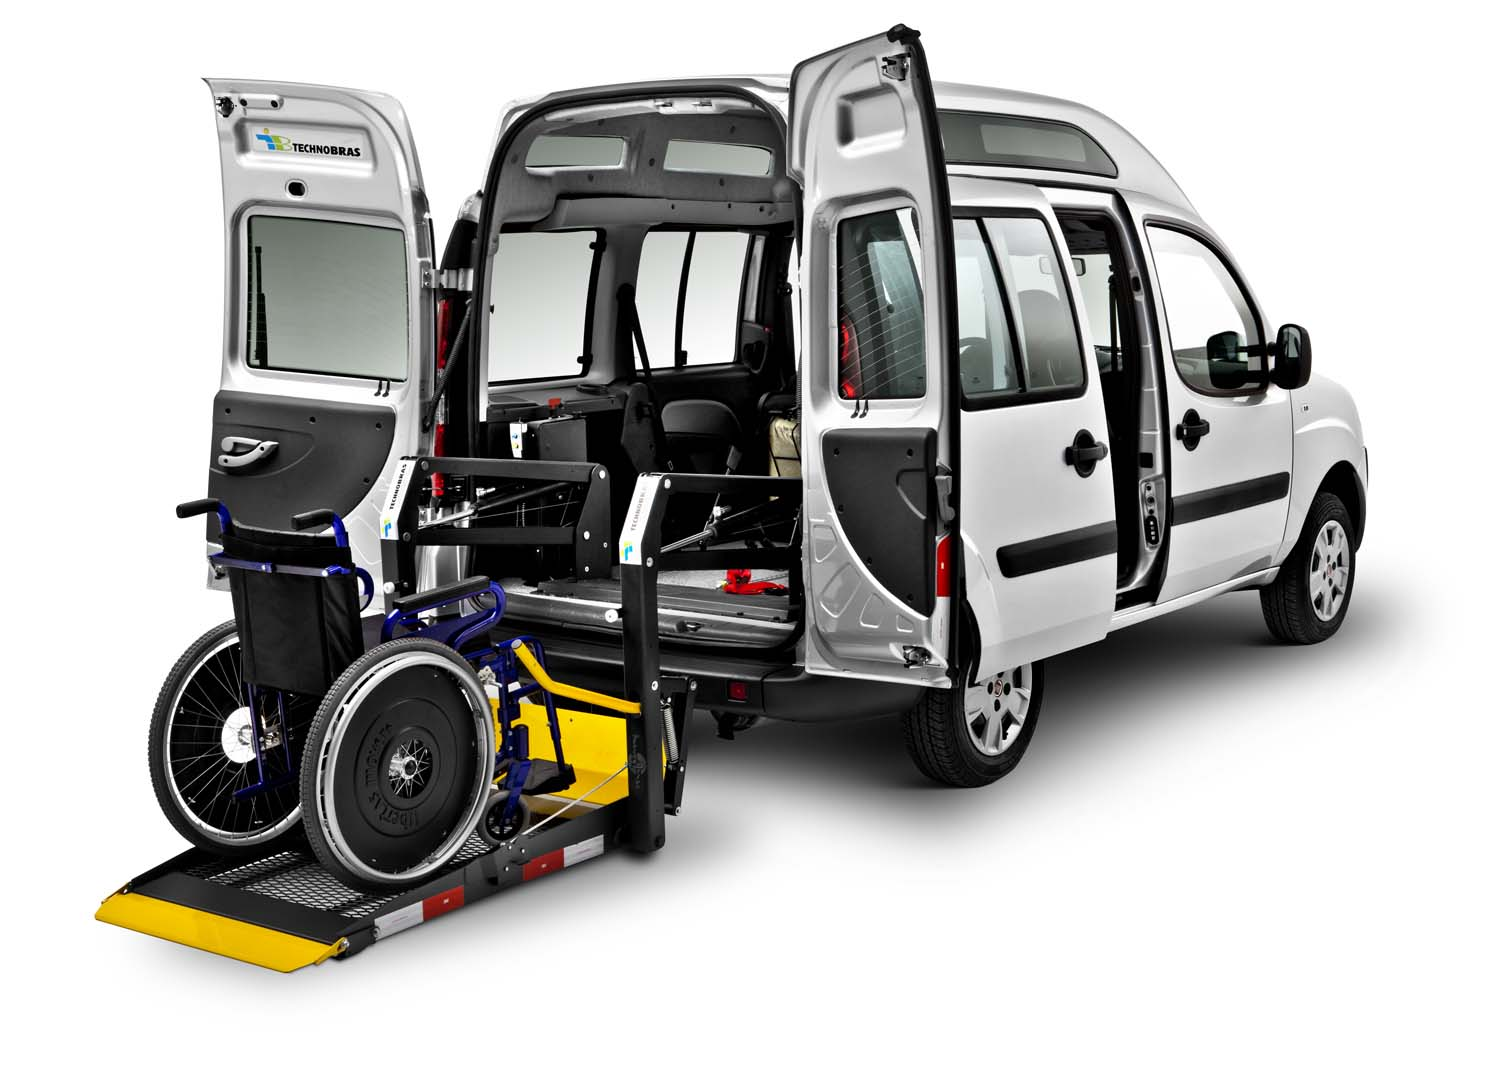
\includegraphics[width=4cm]{../figuras/carro.jpg}\\
			Fonte: \cite{fiat}
    
    \label{fig:carro}
  \end{center}
\end{figure}
}

A Figura \ref{fig:carro} � um exemplo de carro adaptado para pessoas com defici�ncia f�sica, possibilita que estas pessoas possam utilizar um ve�culo autonomamente.


\end{enumerate}


J� segundo a norma ISO 9999:2011(Anexo~\ref{iso9999}), a classifica��o das \ac{TA} se divide em categorias semelhante as diretrizes da \ac{ADA} por�m s�o mais espec�ficas. Para fins te�ricos, � utilizado no trabalho a classifica��o com base nas diretrizes da \ac{ADA} porque al�m da ISO 9999:2011 n�o incluir produtos e equipamentos usados exclusivamente por profissionais de sa�de e dispositivos implantados, a classifica��o \ac{ADA} apresenta um grupo de servi�os de \ac{TA} que promove o apoio � avalia��o da pessoa com defici�ncia, o desenvolvimento e personaliza��o de recursos, a integra��o da \ac{TA} com a��o e objetivos educacionais e de reabilita��o, e os apoios legais de concess�o \cite{corde}.


Uma pesquisa do \ac{W3C} \cite{wc} brasileiro aponta que das pessoas que usam aparelhos de \ac{TA}, 85\% � o computador o dispositivo mais usado, seguido do celular, {\it smarthphone} com 9\%, {\it tablet} com 2\%, e outros dispositivos com 4\%. Sendo cada vez mais necess�rio que existam op��es para esse tipo de p�blico dentro do acesso a informa��o.

A \ac{TA} faz parte da tecnologia, � a parte que auxilia a integra��o das pessoas que possuem algum tipo de defici�ncia. � uma �rea que envolve grandes por��es da popula��o, e que necessita de um cuidado especial, pois envolve al�m da pessoa com defici�ncia, as pessoas nos ambientes em que ela est� inserida.

\subsection{Legisla��o espec�fica de \acf{TA}}

Em rela��o a legisla��o de \ac{TA} alguns decretos s�o relevantes, entre eles a promulga��o do Decreto 3.298 
de 1999, que no artigo 19, fala do direito do cidad�o brasileiro com defici�ncia �s \ac{TA}. 
Nele consta que\cite{lima} (ver anexo {\ref{decreto1}}): 
\begin{quotation}
``Consideram-se ajudas t�cnicas, para os efeitos deste Decreto, os elementos que permitem 
compensar uma ou mais limita��es funcionais motoras, sensoriais ou mentais da pessoa 
portadora de defici�ncia, com o objetivo de permitir-lhe superar as barreiras da comunica��o e da 
mobilidade e de possibilitar sua plena inclus�o social. 
Par�grafo �nico. S�o ajudas t�cnicas:[...]elementos especiais para facilitar a comunica��o, a informa��o e a sinaliza��o para 
pessoa portadora de defici�ncia[...]``
\end{quotation}

O artigo 19 generaliza o termo Ajudas T�cnicas a todos os elementos que compensam limita��es do ser humano, por�m sem caracteriza��o ou classifica��o objetiva de tais ajudas. Tamb�m relevante, o decreto 5.296 de 2002, que d� prioridade de atendimento e estabelece normas gerais e crit�rios b�sicos para a promo��o da acessibilidade das pessoas com defici�ncia ou com 
mobilidade reduzida, possui um cap�tulo espec�fico sobre as ajudas t�cnicas no qual descreve 
v�rias inten��es governamentais na �rea da \ac{TA}, al�m de referir a constitui��o do 
\ac{CAT}. Neste decreto encontra-se que\cite{lima}: 
\begin{quotation}
``Consideram-se ajudas t�cnicas os produtos, instrumentos, equipamentos ou tecnologia 
adaptados ou especialmente projetados para melhorar a funcionalidade de pessoas portadoras de  
defici�ncia, com habilidade reduzida favorecendo autonomia pessoal, total ou assistida" .
\end{quotation}

No decreto 5.296\cite{cata} a legisla��o cita ao inv�s da compensa��o como no artigo 19, a autonomia total ou assistida das pessoas com defici�ncia. Embora esse Comit� leve a express�o ``Ajudas T�cnicas'' em sua 
denomina��o, tamb�m porque � a express�o prevista na legisla��o brasileira, 
os estudos desenvolvidos apontam e sugerem que as express�es 
``Tecnologia Assistiva'', ``Ajudas T�cnicas'' e ``Tecnologia de Apoio'', neste 
momento, continuem sendo entendidas como sin�nimos e que correspondam 
�s bases conceituais aprovadas pelo Comit�. Entretanto, estabelece a 
utiliza��o �nica da express�o ``Tecnologia Assistiva'' em seus documentos, 
como a mais apropriada, pelos seguintes motivos \apud{cata}{galvao}: 
\begin{itemize}
 
\item Por ser uma tend�ncia nacional j� firmada no meio acad�mico, nas 
organiza��es de pessoas com defici�ncia, em setores governamentais 
(Minist�rio MEC da Educa��o, Minist�rio da Ci�ncia e Tecnologia (MCT), Conselho Nacional de Desenvolvimento Cient�fico e Tecnol�gico CNPq), Institutos de Pesquisa (ITS Brasil) e no mercado de produtos; 
 
\item Pelo primeiro objetivo do Comit� de Ajudas T�cnicas, expl�cito no Artigo 
66 do Decreto 5296/2004, relativo � estrutura��o das diretrizes da �rea 
do conhecimento. A express�o Tecnologia Assistiva seria a mais 
compat�vel como a denomina��o de uma �rea de conhecimento, a ser 
oficialmente reconhecida; e
 
\item Por ser uma express�o bastante espec�fica ao conceito ao qual 
representa, diferentemente das express�es ``Ajudas T�cnicas'' e 
``Tecnologia de Apoio'', que s�o mais gen�ricas e tamb�m utilizadas para 
referirem-se a outros conceitos e realidades diferentes. 
\end{itemize}

Conforme votado e aprovado por unanimidade na quinta Reuni�o desse Comit�, al�m da determina��o de utiliza��o �nica da express�o Tecnologia Assistiva, foi decidido tamb�m que essa express�o seja utilizada no singular, por referir-se a uma �rea do conhecimento e sugere-se que se fa�am os poss�veis encaminhamentos para a revis�o da nomenclatura em 
instrumentos legais no pa�s. Este mesmo Comit� de Ajudas T�cnicas tamb�m aprovou, na sua terceira Reuni�o de abril de 2007, as bases conceituais que situam a Tecnologia Assistiva nos seguintes marcos \cite{cata,catb}: 

\begin{itemize}
\item �rea do Conhecimento;
\item Multidisciplinariedade;
\item Objetivos: promover a funcionalidade (atividade, participa��o) de 
pessoas com defici�ncia, mobilidade reduzida, ou idosas, visando sua 
autonomia, independ�ncia, qualidade de vida e inclus�o social; 
\item Composi��o: produtos, recursos, estrat�gias, pr�ticas, processos, 
m�todos e servi�os; e 
\item Ter presente os princ�pios do {\it Universal Design}\footnote{O conceito de Desenho Universal, ou ``{\it Universal Design}'', ou tamb�m chamado ``Desenho para todos'', � estudado a partir de alguns princ�pios tais como: equipara��o nas possibilidades de uso; flexibilidade no uso; uso simples e intuitivo; capta��o da informa��o; toler�ncia ao erro: m�nimo esfor�o f�sico; dimens�o e espa�o para uso e intera��o \cite{sepro}} e ITS BRASIL (Instituto de Tecnologia Social).

\end{itemize}

Apesar de uma iniciativa e uma legisla��o recente os assuntos acessibilidade e ajudas t�cnicas vem entrando no cotidiano dos brasileiros, pois h� uma cobran�a da parte governamental. Por�m, ainda existe uma defici�ncia em normas e na pr�pria legisla��o que regulamente as \ac{TA} principalmente na parte de classifica��o e exig�ncias.

\subsection{Iniciativas de \ac{TA}}
\label{iniciativas}

Existem v�rias iniciativas de \ac{TA} pelo mundo, como a  Funda��o SIDAR\cite{sidar} ({\it Seminario Iberoamericano sobre Diversidad y Accesibilidad en la Red}) que � uma institui��o de observa��o e recomenda��o na �rea da acessibilidade e inclus�o digital para os territ�rios ibero-americanos, a ATI\cite{ati} ({\it Assistive Technology Initiative}) na Universidade De George Mason na Virg�nia nos Estado Unidos, o INCNESI\cite{incnesi} (Iniciativa Nacional para os Cidad�os com Necessidades Especiais na Sociedade da Informa��o) que incentiva o uso de equipamentos para pessoas com defici�ncia em Portugal. 

Ainda no �mbito europeu, em 1999 foi organizado o Cons�rio \ac{EUSTAT} que desenvolveu um estudo entre 1997 e 1999, no contexto do Programa de Aplica��es Telem�ticas da Comiss�o Europeia, destinado a forma��o de usu�rios finais de \ac{TA}, envolvendo pessoas com defici�ncia ou idosos, seus familiares e profissionais assistentes pessoais, para que os mesmos pudessem fazer escolhas informadas, adequadas e respons�veis em rela��o a essas tecnologias. Esse estudo parte do princ�pio de que � fundamental a participa��o de usu�rio final como parceiro ativo na escolha das \ac{TA} que utiliza\cite{galvao}.

S�o parceiros do Cons�rcio \ac{EUSTAT} as seguintes organiza��es \cite{eustat}:

\begin{itemize}

\item SIVA {\it Servizio Informacione e Valutazione Ausili da Fondazione Dom Carlo Ghocchi Onlus}, da It�lia. Possui um centro de Inova��o e Transfer�ncia de Tecnologia, que incentiva projetos para autonomia de pessoas com defici�ncias;

\item CAPS  Centro de An�lise e Processamento de Sinais, do Instituto Superior T�cnico de Lisboa, Portugal;

\item \it{Association Nationale pour le Logement des personnes handicap�es}, da B�lgica;

\item \it{Groupement pour l�insertion des personnes handicap�es physiques}, da Fran�a;

\item \it{Danish Centre for Technical Aids for Rehabilitation and Education}, da Dinamarca; e

\item \it{Centro Studi Prisma}, da It�lia.

\end{itemize}

Os estudos que s�o parceiros do cons�rcio, s�o centros de refer�ncia em \ac{TA} na Europa, juntas s�o respons�veis por uma parte consider�vel de publica��es, dispositivos, sobre \ac{TA}. O Cons�rcio EUSTAT recomenda a classifica��o \ac{HEART} que prop�e tr�s grandes �reas de forma��o em 
rela��o �s \ac{TA}:
\begin{itemize} 
\item Componentes t�cnicos;
\item Componentes humanos; e
\item Componentes socioecon�micos.
\end{itemize}

Essa classifica��o tem ganhado for�a na atualidade, principalmente em decorr�ncia do paradigma inclusivo, o qual desloca as limita��es de funcionalidade e possibilidades de participa��o do �mbito restrito � defici�ncia em si, para situ�-las a partir das barreiras impostas pelo ambiente f�sico e social\cite{rodrigues}. Como n�o foi encontrado uma padroniza��o mundial para a defini��o de \ac{TA} as diferentes iniciativas encontradas se relacionam na tabela \ref{tabeladois}.

\begin{table}[bth!]
\centering
\scriptsize
\caption{Tabela com as diferen�as de Iniciativas de \ac{TA} encontradas.}\vspace{.2cm}
 \begin{tabular}{|p{2cm} |  p{3.9cm} | p{3cm} | p{4cm}| }
    \hline
    Pa�s & Termo Utilizado (Tradu��o) & Classifica��o & Defini��o \\ \hline
    Brasil & Tecnologia Assistiva, Ajudas T�cnicas &Ca\-te\-go\-ri\-as relativas aos e\-qui\-pa\-men\-tos & Melhorar as pessoas com defici�ncia e mobilidade re\-du\-zi\-da \\ \hline
    EUTSTAT & Ajudas T�cnicas e Tecnologia de Apoio & Classifica��o por componentes& Compensar as pessoas com defici�ncia e idosas \\ \hline
    ADA & {\it Assistive Technology} (Tecnologia Assistiva) & Trata as situa��es & Ajudas aos indiv�duos com defici�ncia em situa��es es\-pe\-c�\-fi\-cas \\ \hline	
		\end{tabular}
    \label{tabeladois}
		\\Fonte: o pr�prio autor.

\end{table}

A tabela {\ref{tabeladois}} mostra as diferen�as das tr�s iniciativas mais relevantes encontradas. Apesar da mudan�a de termos, as iniciativas n�o possuem grandes diferen�as entre si. A classifica��o da \ac{TA} � o �nico fator que diferencia nas iniciativas. Por�m, a relev�ncia da mudan�a � pequena, em rela��o a as ajudas �s pessoas com defici�ncia.


\section{Comunica��o Alternativa Ampliada (CAA)}

Na \ac{TA}, como mencionado anteriormente na se��o {\ref{Tecnologia Assistiva}} se divide em algumas classifica��es, dentro delas temos a \ac{CAA}, que � linha de pesquisa adotada neste trabalho. A \ac{CAA} abrange qualquer meio de comunica��o que suplemente ou substitua os m�todos naturais de fala ou escrita. � um meio que auxilia a comunica��o de um indiv�duo com outras pessoas. Os sistemas de \ac{CAA} podem ser divididos em pictoriais\footnote{Os sistemas pictoriais representam os referentes por analogia f�sica e n�o por conven��o arbitr�ria, o que lhes confere iconicidade e clareza denotativa, sendo bem compreendidos, aprendidos e lembrados por crian�as, estrangeiros e c�rebro-lesados. Contudo, o universo de significados que podem representar restringe-se ao imagin�vel \cite{fernando}.} e simb�licos\footnote{Os sistemas simb�licos representam referentes por conven��es arbitr�rias, usando regras de recombina��o e sintaxe espec�fica, o que resulta em opacidade denotativa, mas lhes permite representar virtualmente qualquer conceito, imagin�vel ou n�o \cite{fernando}.} podendo ser de alta tecnologia (e.g., sistemas computadorizados, e softwares especiais) e baixa tecnologia (e.g., simples, e n�o el�tricos) \cite{leydi}.

A \ac{CAA} � definida como uma maneira alternativa � comunica��o oral e escrita que compreende o uso de gestos, sinais manuais, express�es faciais, pranchas com s�mbolos pictogr�ficos, pranchas de alfabeto, comunicadores de voz gravada ou sintetizada at� sistemas sofisticados de computador \apud{glennen}{correia}. Inicialmente eram utilizados sistemas sem tecnologia, recorrendo apenas ao corpo humano, como a linguagem por sinais (e.g., libras) passando pelos sistemas anal�gicos ou de baixa tecnologia (e.g., cart�es e livros com s�mbolos e imagens) at� sistemas baseados em recursos computacionais (e.g., vocalizadores, e softwares para computador com s�ntese de voz) \apud{worthy}{correia}.

O trabalho da \ac{CAA} engloba uma s�rie de s�mbolos, recursos, estrat�gias e t�cnicas para auxiliar o desenvolvimento de uma comunica��o complementar. Os s�mbolos s�o as representa��es visuais, auditivas ou t�teis de um conceito; os recursos s�o os objetos ou equipamentos utilizados para transmitir as mensagens que podem ser pranchas de comunica��o, os comunicadores ou o computador; as t�cnicas s�o as formas como as mensagens s�o transmitidas e as estrat�gias referem-se ao modo como os recursos da \ac{CA} s�o utilizados \apud{king}{pelosi2}.

Como o foco deste trabalho � encontrar uma solu��o alternativa a pessoas que possuem defici�ncia na fala, em conjunto com defici�ncia motora (quadros tabela cl�nicos), a \ac{CAA} � a abordagem encontrada que melhor se encaixa neste contexto. Pois a \ac{CAA} utiliza estrat�gias e t�cnicas para o desenvolvimento de uma comunica��o complementar, que auxiliam a suplementa��o ou substitui��o da forma natural de comunica��o.


\section{Considera��es do Cap�tulo}

Com a pesquisa realizada no cap�tulo {\ref{cap:introducao}}, fica evidenciado que pessoas com necessidades especiais, precisam de recursos que supram ou compensem suas defici�ncias para que possam ser inseridas na sociedade. Apesar de uma por��o consider�vel da popula��o mundial possuir algum tipo de defici�ncia, os estudos e legisla��o sobre a \ac{TA} s�o consideravelmente recentes.
	
Al�m disso, vale ressaltar a import�ncia de que se desenvolva mais solu��es de \ac{TA}, principalmente acess�veis, e que os desenvolvedores, se preocupem com o ambiente em que esta pessoa est� inserida e as pessoas com as quais ela ir� interagir. Foram necess�rios conhecimentos sobre \ac{TA}, \ac{CAA} e acessibilidade para que se entenda o foco deste trabalho que visa encontrar uma solu��o alternativa de \ac{CAA} para pessoas que possuem \ac{PC} que apresentam defici�ncia motora e de fala.
	
Este trabalho se enquadra na Lei no 10.098, de dezembro de 2000 que estabelece crit�rios como o artigo 17 que garante direito de comunica��o e express�o por mecanismos, ou alternativas t�cnicas. Al�m disso, se enquadra tamb�m, no Decreto 5296/2004, Artigo 66 do Comit� de Ajudas T�cnicas, no qual estabelece o termo \acf{TA} como a denomina��o mais compat�vel ao tema.

O trabalho tamb�m pode ser classificado nas diretrizes da \ac{ADA} como um trabalho no contexto de \acf{CAA}. J� na norma ISO 9999:2011 na subcategoria, Produtos de Apoio para Treino de Comunica��o Alternativa e Aumentativa, c�digo 05 06 27, categoria Produtos de apoio para treino de comunica��o com imagens e desenhos.

\chapter{Referencial Te�rico}
\label{cha:refTeorico}
Apresentar todas as tecnolonologias utilizadas para o desenvolvimento do trabalho

\section{Entrada de S�mbolos e Siglas}
Para fazer a entrada de um s�mbolo, $\backslash$s�mbolo\{\simbolo{$\sigma$}{Descri��o}\} \{sigma\} � a forma correta. E, para definir uma sigla, $\backslash$sigla\{\sigla{ABNT}{Associa��o Brasileira de Normas T�cnicas}\} \{Descri��o\} deve ser utilizado.

Obs.: Quando a sigla ou o s�mbolo aparecerem novamente no texto, n�o repita o comando, para que a sigla ou s�mbolo n�o se repita na lista correspondente.

\section{Introdu��o � tecnologia X}


Inserindo uma referencia da tecnologia x \cite{ref}.


Exemplo para inserir figura. Figura \ref{fig:nomeParaRef}.


\begin{figure}[!htb]
	\centering
	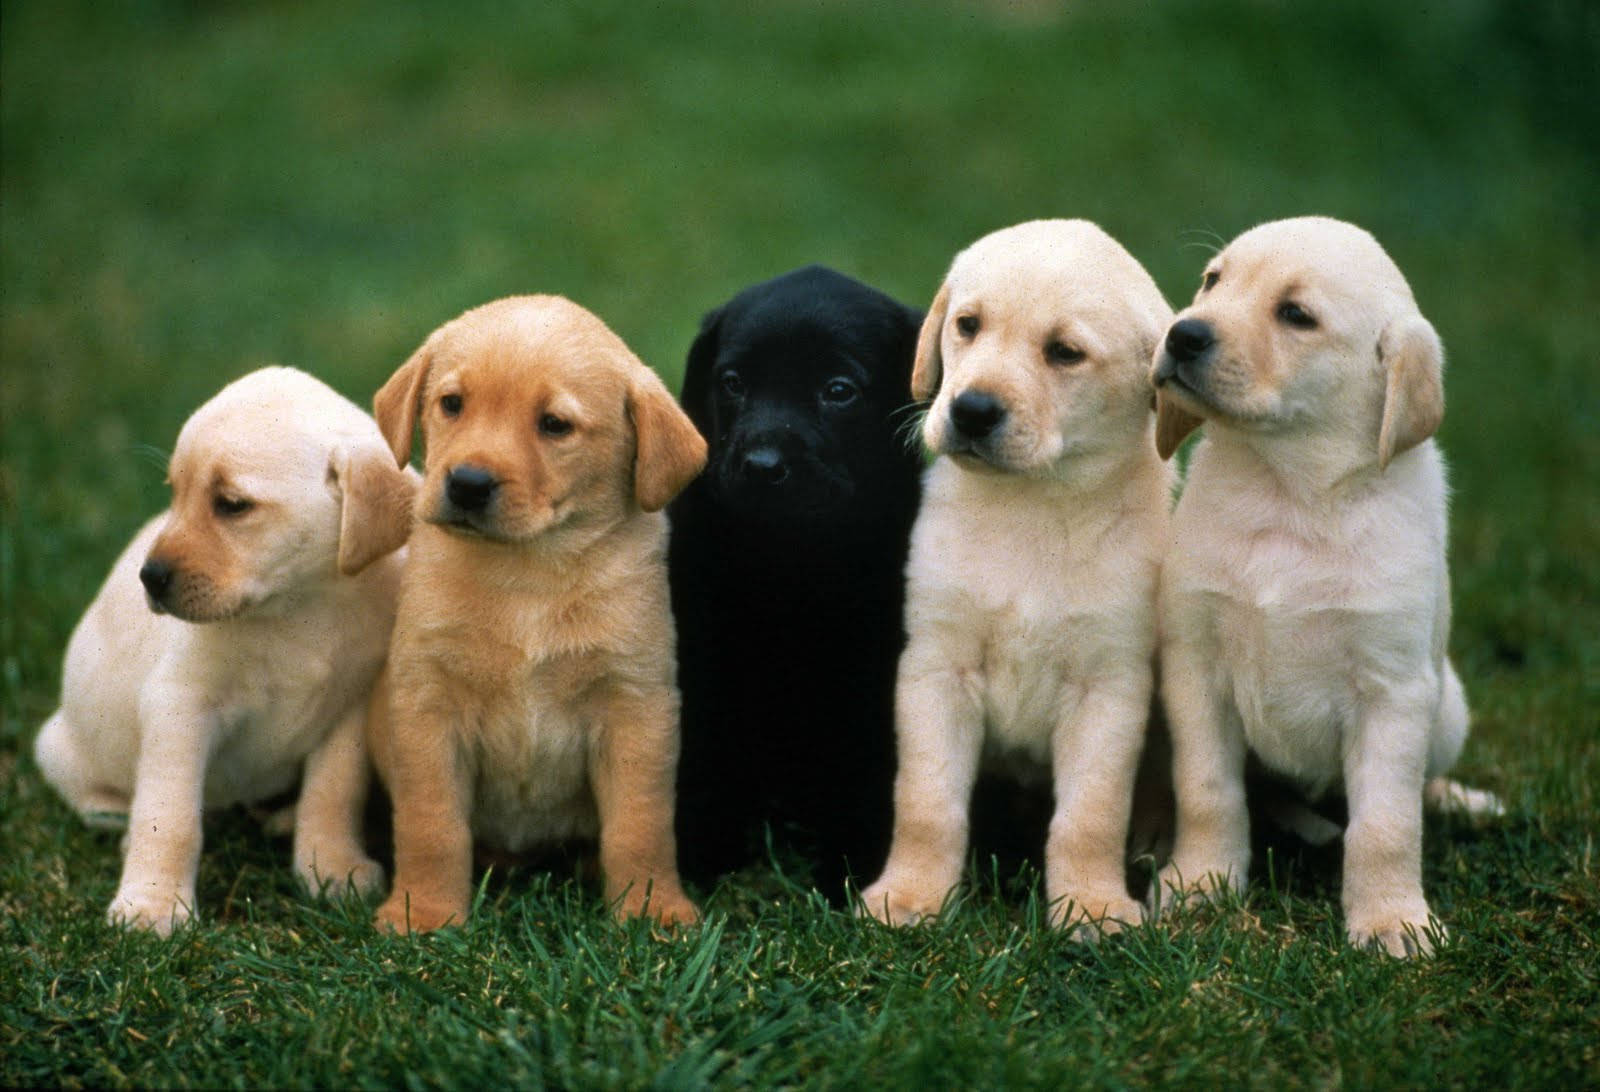
\includegraphics[width=0.45\textwidth]{../5_figuras/fig1}
	\caption{T�tulo da figura}
	\label{fig:nomeParaRef}
\end{figure}


exemplo de figura lado a lado. Figura \ref{fig:a} e \ref{fig:a}

\begin {figure}[htbp]
	\begin {center}
    \subfloat [Figura a]{
    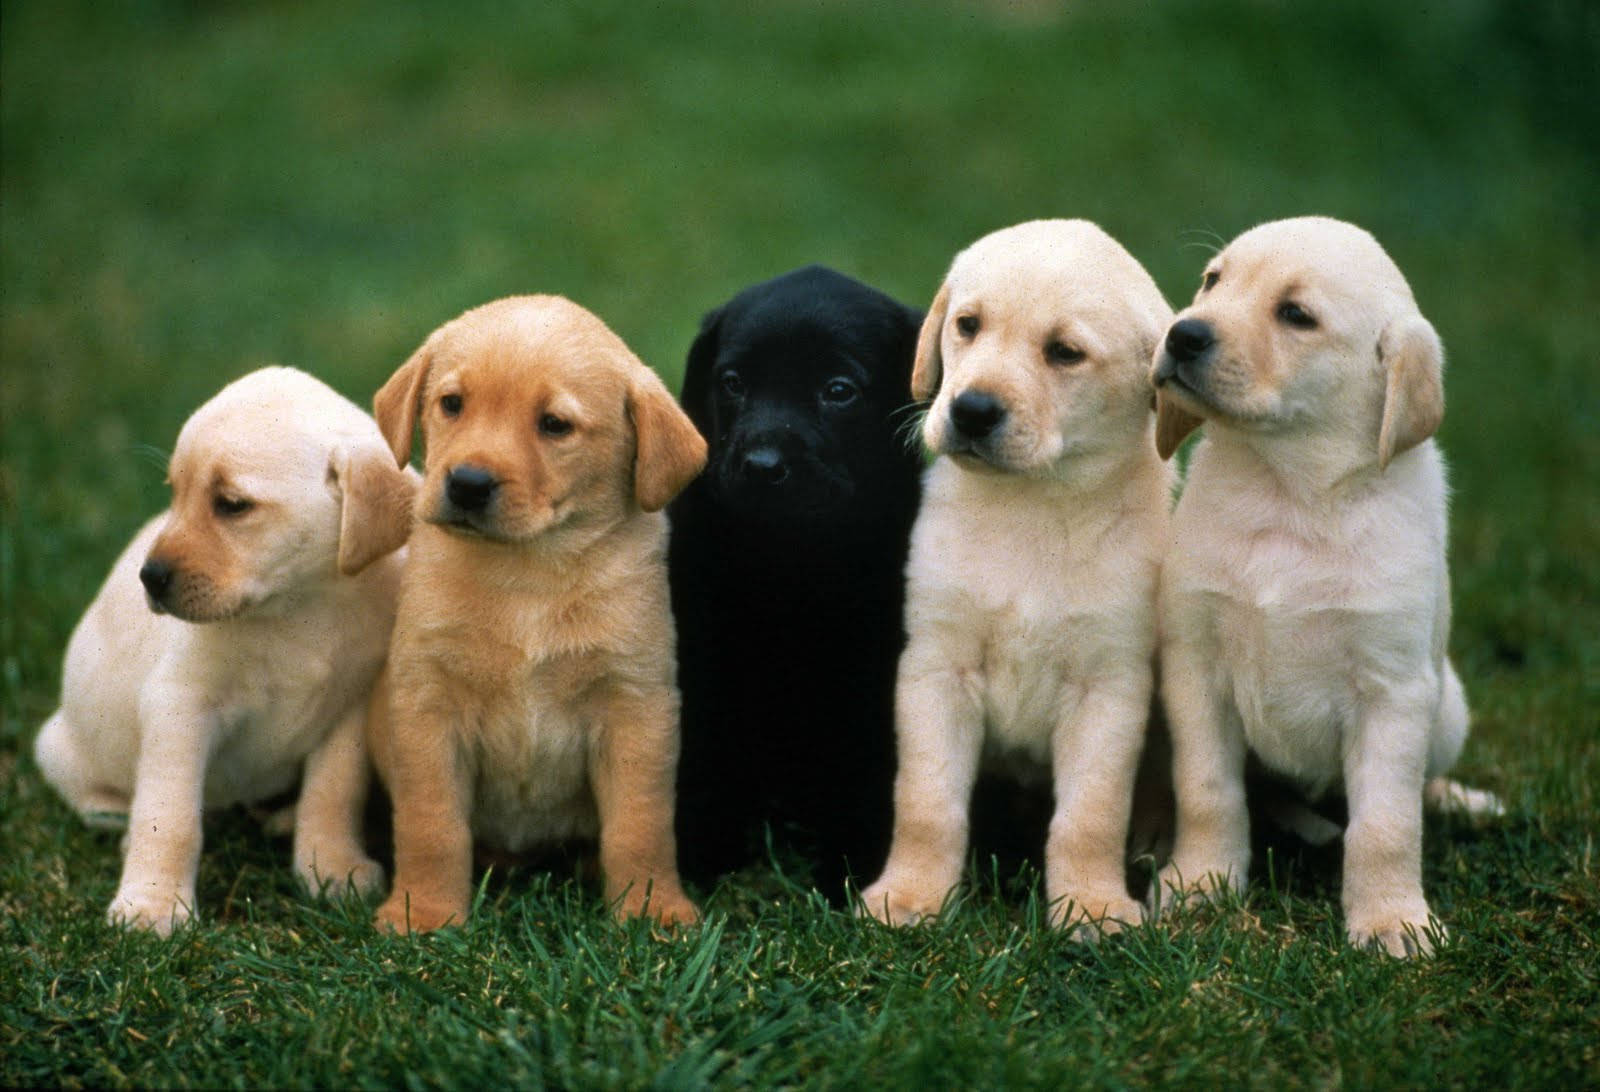
\includegraphics[width=0.35\linewidth]{../5_figuras/fig1}
    \label{fig:a}
    }
    \subfloat [Figura b]{
    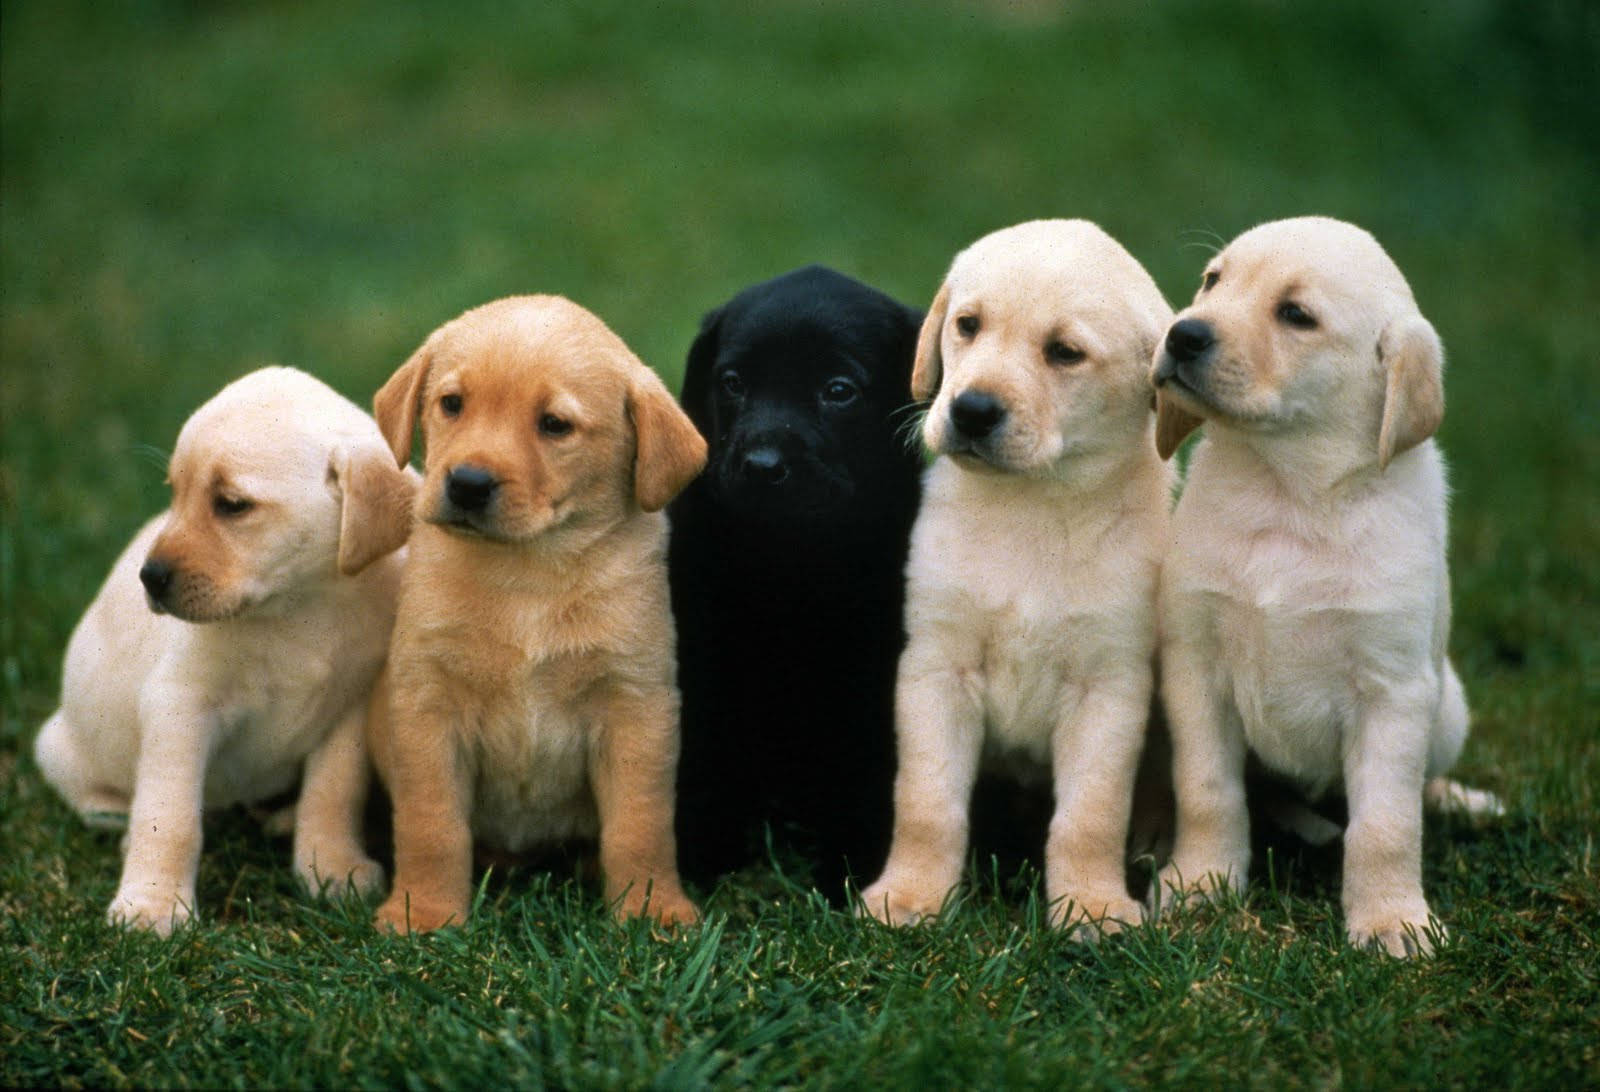
\includegraphics[width=0.35\linewidth]{../5_figuras/fig1}
    \label{fig:b}
    }
    \caption{itulo}
    \end{center}
\end{figure}

\section{Conclus�es do cap�tulo}
\chapter{Trabalhos Relacionados}
\label{cha:relacionados}
Apresentar os principais trabalhos relacionados.

\section{Trabalho 1}

Descrever o trabalho 1.

\section{Trabalho 2}

Descrever o trabalho 2.

\section{Conclus�es do cap�tulo}

Exemplo para inserir tabela. Tabela \ref{tb:nomeParaRef}

\begin{table}[!htb]
\caption{T�tulo da Tabela}
\label{tb:nomeParaRef}
\begin{center}
\begin{tabular}{l c c} \hline
Trabalhos  & Caracter�stica 1 & Caracter�stica 2 \\ \hline 

Trabalho 1 & Sim/N�o          & Sim/N�o          \\ \hline

Trabalho 2 & Sim/N�o          & Sim/N�o          \\ \hline

\end{tabular}
\end{center}
\end{table}
\chapter{Proposta}
\label{cha:proposta}
Apresentar a proposta do trabalho

\section{Vis�o geral}


\section{Conclus�es do cap�tulo}
\chapter{Avalia��o de desempenho}
\label{cha:resultados}


\section{Caso de Uso}

\section{Descri��o da simula��o}

\section{Analise dos resultados}

\section{Conclus�es do Cap�tulo}
\chapter{Conclus�es}
\label{cha:conclusao}


\bibliographystyle{abnt}%template de referencia da ABNT
%\bibliographystyle{IEEEtran}%template de referencia do IEEE
%\bibliographystyle{sbc} %template de referencia do SBC
\bibliography{../4_pos_texto/biblio}

% *********** AP�NDICES ***********
% ** Condicionados � necessidade **
\appendix
\chapter{Ap�ndice}
\renewcommand{\thesection}{\Alph{section}}
\section{Quadros Cl�nicos de Paralisia Cerebral}
\label{apendice1}
\begin{enumerate}
\item {Hemiplegia : � a manifesta��o mais frequente, com
maior comprometimento do membro superior;
acompanha-se de sinais de libera��o tais como
espasticidade , hiper reflexia e sinal de Babinski. O
paciente assume atitude em semiflex�o do membro
superior, permanecendo o membro inferior
hiperestendido e aduzido, e o p� em postura equinovara.
� comum hipotrofia dos segmentos acometidos, sendo
tamb�m poss�vel a ocorr�ncia de outras hemi-hipoestesia
ou hemianopsia.}
\item{ Hemiplegia bilateral ( tetra ou quadriplegia) :
Ocorrem de 9 a 43\% dos pacientes. Ocorrem les�es
difusas bilateral no sistema piramidal dando al�m da
grave tetraparesia esp�stica com intensas retra��es em
semiflex�o, s�ndrome pseudobulbar (hipomimia, disfagia
e disartria), podendo ocorrer ainda microcefalia,
defici�ncia mental e epilepsia.}
\item{Diplegia : Ocorre em 10 a 30 \% dos pacientes, sendo
a forma mais encontrada em prematuros. Tratase de um
comprometimento dos membros inferiores, comumente
evidenciando uma acentuada hipertonia dos adutores,
que configura em alguns doentes o aspecto semiol�gico
denominado s�ndrome de Little (postura com cruzamento
dos membros inferiores e marcha em tesoura). H� 
diferentes grada��es quanto � intensidade do dist�rbio,
podendo ser pouco afetado (tendo recupera��o e bom
progn�stico  adaptam-se � vida di�ria); enquanto outros
evoluem mal com graves limita��es funcionais. Os dados
semiol�gicos s�o muito vari�veis. No 1� ano de vida, a
crian�a apresenta-se hipot�nica, evoluindo
gradativamente para uma outra fase em que se observa
um quadro de distonia intermitente, com tend�ncia ao
opist�tono quando estimulada. Nos casos mais graves a
crian�a pode permanecer num destes est�gios por toda
a sua vida, por�m geralmente passa a exibir hipertonia
esp�stica, inicialmente extensora e, finalmente, com
graves retra��es semiflexoras.}
\item{Discinesia : Atualmente � a mais rara, pois
manifesta-se atrav�s de movimentos involunt�rios,
sobretudo distonias axiais e/ou movimentos c�reoatet�ides
das extremidades. No primeiro ano de vida este
padr�o costuma n�o estar definido, podendo existir
hipotonia muscular. Em geral, quando estes pacientes
est�o relaxados a movimenta��o passiva � facilitada.}
\item{Ataxia : Igualmente rara. Inicialmente pode traduzir se
por hipotonia e, aos poucos, verificam-se altera��es
do equil�brio (ataxia axial) e, menos comumente, da
coordena��o ( ataxia apendicular). Sua marcha se faz com
aumento da base de sustenta��o podendo apresentar
tremor intencional.}
\item{Formas mistas : � a associa��o das manifesta��es
anteriores, correspondendo, geralmente, ao encontro de
movimentos dist�nicos e c�reo atet�ides ou �
combina��o de ataxia com plegia (sobretudo diplegia).
No total, cerca de 75\% dos pacientes doentes com
paralisia cerebral apresentam padr�o esp�stico.
Al�m do dist�rbio motor, obrigat�rio para a
caracteriza��o da paralisia cerebral, o quadro cl�nico pode
incluir tamb�m outras manifesta��es acess�rias com
frequ�ncia vari�vel: 
\begin{enumerate}
\item{ Defici�ncia mental: Ocorre de 30 a
70\% dos pacientes. Est� mais associada �s formas
tetrapl�gicas, dipl�gicas ou mistas;}
\item{ Epilepsia: Varia de
25 a 35\% dos casos, ocorrendo mais associado com a
forma hemipl�gica ou tetrapl�gica; }
\item{ Dist�rbios da
linguagem; }
\item{ Dist�rbios visuais : Pode ocorrer perda da
acuidade visual ou dos movimentos oculares
\(estrabismo\); }
\item{ Dist�rbios do comportamento : S�o mais
comuns nas crian�as com intelig�ncia normal ou lim�trofe,
que se sentem frustradas pela sua limita��o motora,
quadro agravado em alguns casos pela super prote��o
ou rejei��o familiar; e}
\item{ Dist�rbios ortop�dicos : Mesmo
nos pacientes submetidos � reabilita��o bem orientada,
s�o comuns retra��es fibrotend�neas \(50\%\) cifoescoliose
\(15\%\), coxa valga \(5\%\) e deformidades nos p�s.
Todos esses dist�rbios se d�o devido a altera��es
nas �reas motoras cerebrais espec�ficas durante a
inf�ncia.}
\end{enumerate}
}
\end{enumerate}
\newpage
\section{Entrevista}
\label{entrevista}
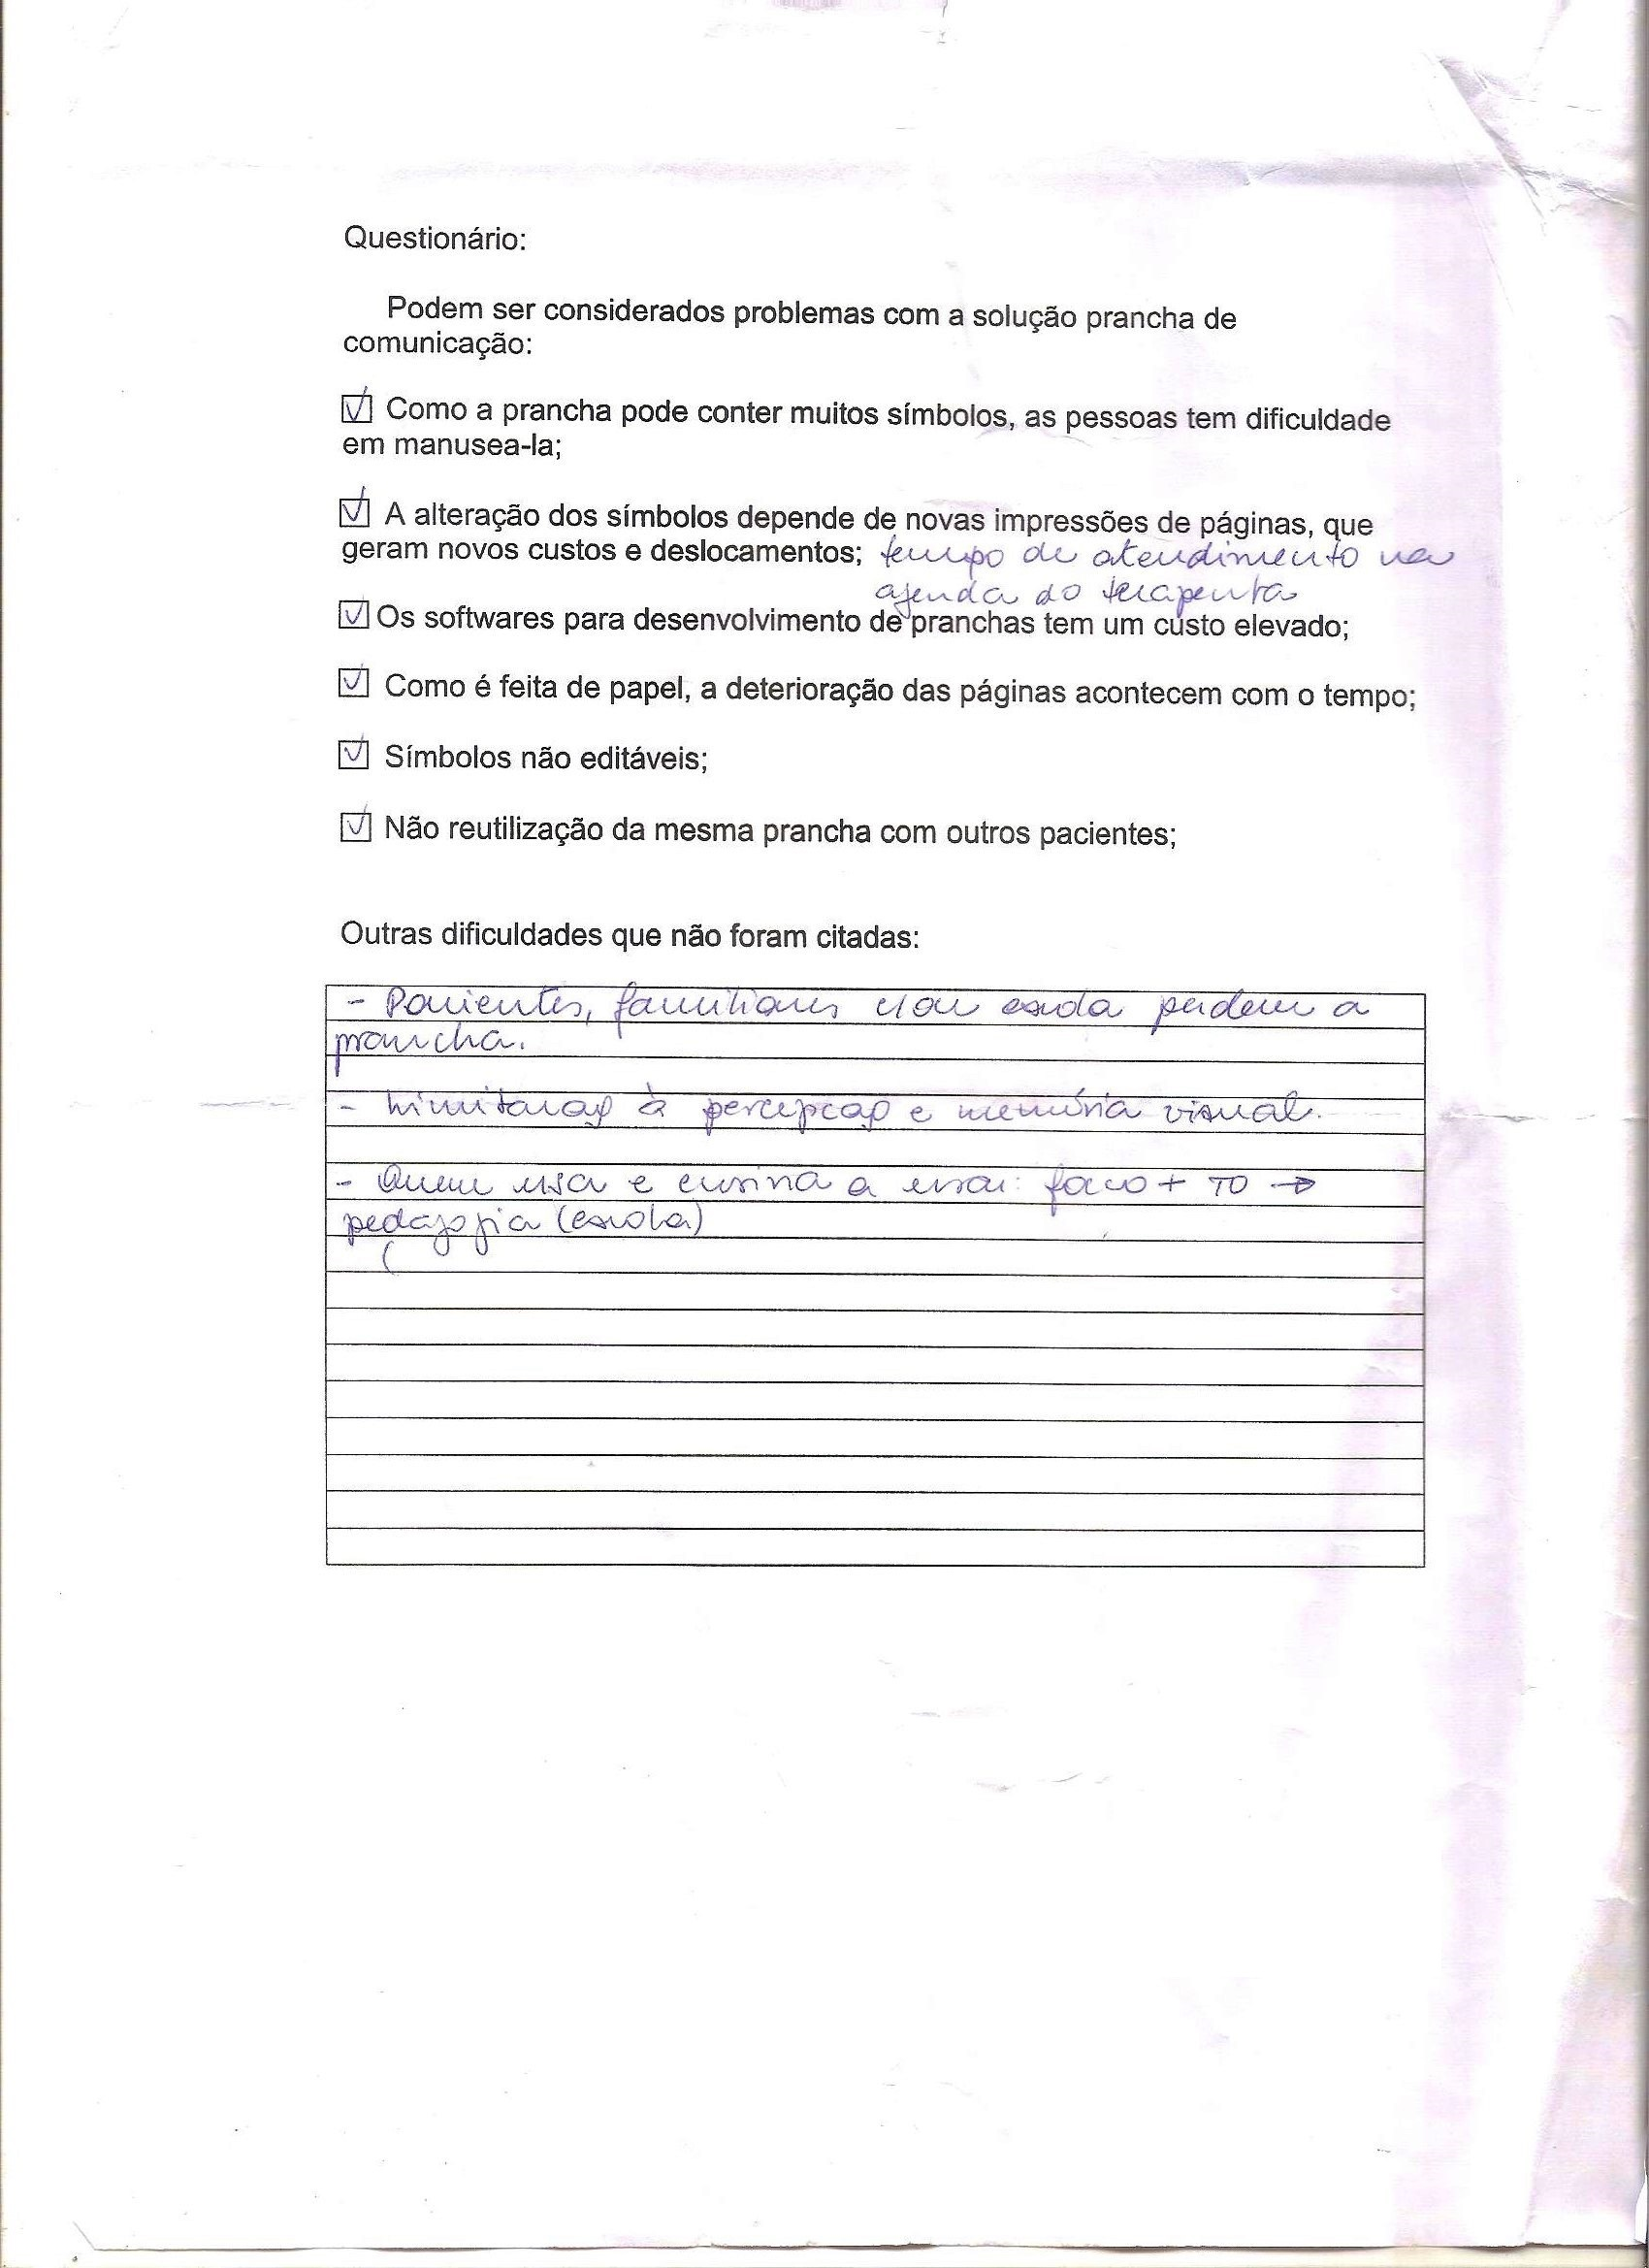
\includegraphics[scale=0.8]{../figuras/entrevista.jpg}


% ************ ANEXOS *************
% ** Condicionados � necessidade **
\anexo
\chapter{Primeiro anexo}

 Anexos s�o documentos n�o elaborados pelo autor, que servem de fundamenta��o, comprova��o ou ilustra��o.





\end{document}
